\documentclass{beamer}
\usepackage[english, russian]{babel}
\usepackage[T2A]{fontenc}
\usepackage[utf8]{inputenc}
\usepackage{indentfirst}
\usepackage{amsmath, amsfonts, amssymb, amsthm, mathtools}
\usepackage[export]{adjustbox}
\usepackage{graphicx} 
\graphicspath{ {./images/} }

\usepackage{subcaption}
\usepackage{verbatim}

\usepackage{minted}{\setlength{\parskip}{0pt}}

\usepackage{hyperref}

\hypersetup{
    colorlinks=true,
    linkcolor=blue,
    filecolor=magenta,      
    urlcolor=black,
    pdftitle={Overleaf Example},
    pdfpagemode=FullScreen,
    }


\title{Отчет по лабораторной работе № 11. \\ Настройка безопасного удалённого доступа по протоколу SSH}
\author{Данила Стариков \\ НПИбд-02-22}
\date{2024}

\begin{document}

\maketitle
\newpage

\tableofcontents

\newpage
\section{Цель работы}
Приобретение практических навыков по настройке удалённого доступа к серверу с помощью SSH.

\newpage
\section{Выполнение работы}
\subsection{Запрет удалённого доступа по SSH для пользователя root}
\begin{enumerate}
\item На сервере задали пароль для пользователя root (Рис. \ref{01}):
  \begin{minted}{bash}
    sudo -i
    passwd root
  \end{minted}
\begin{center}
  \centering
  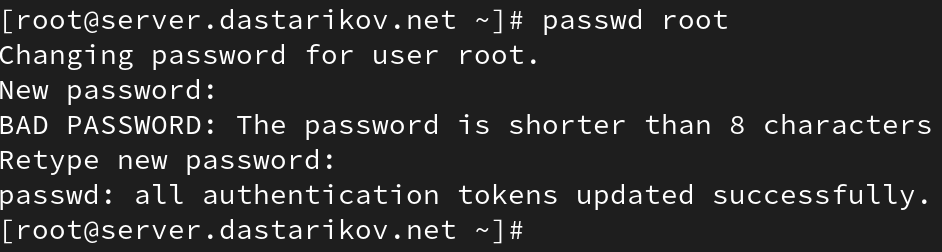
\includegraphics[width=\textwidth]{../images/image01.png}
  \captionof{figure}{Задание пароля для пользователя root.}
  \label{01}
\end{center}

\item На сервере в дополнительном терминале запустили мониторинг системных событий:
  \begin{minted}{bash}
    sudo -i
    journalctl -x -f
  \end{minted}
\item С клиента попытались получить доступ к серверу посредством SSH-соединения через пользователя \texttt{root} (Рис. \ref{02}):
  \begin{minted}{bash}
    ssh root@server.dastarikov.net
  \end{minted}
\begin{center}
  \centering
  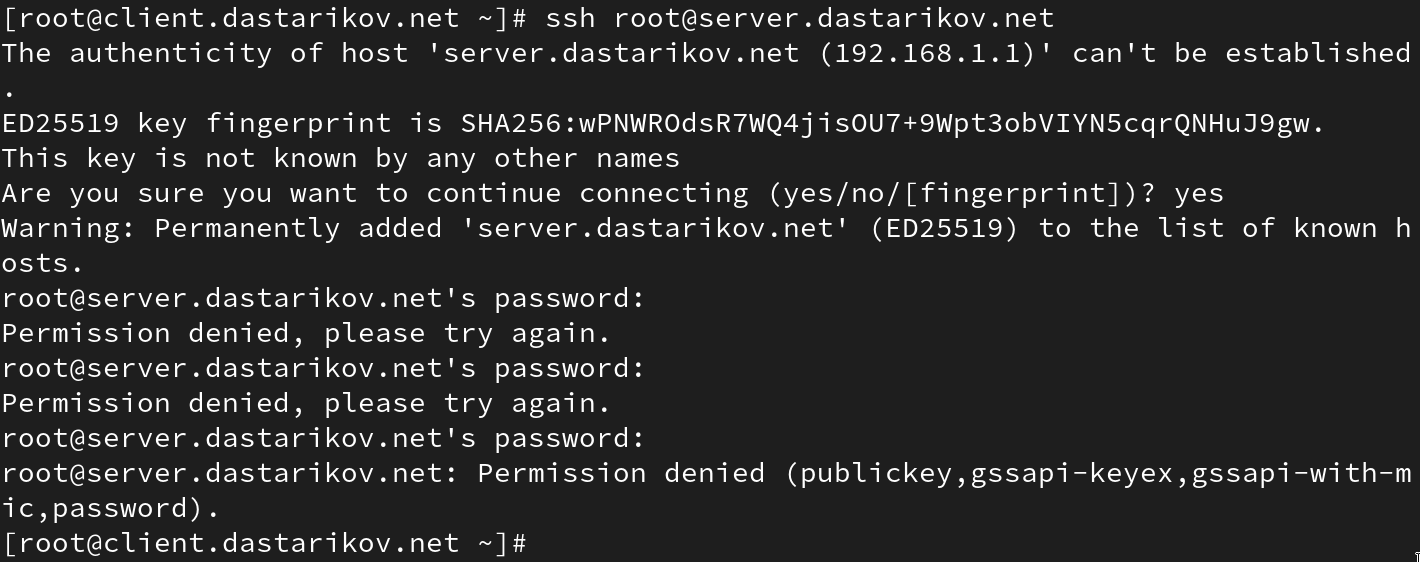
\includegraphics[width=\textwidth]{../images/image02.png}
  \captionof{figure}{Подключение к серверу через SSH-соединение.}
  \label{02}
\end{center}

Несмотря на правильно введенный пароль для пользователя root, не получилось подключиться, так как в конфигурации ssh запрещен подключение для пользователя root с помощью пароля (по умолючанию используется настройка \texttt{PermitRootLogin prohibit-password}).

\item На сервере открыли файл \texttt{/etc/ssh/sshd\_config} конфигурации \texttt{sshd} для редактирования и запретили вход на сервер пользователю \texttt{rootf}, установив:
  \begin{minted}{bash}
    PermitRootLogin no
  \end{minted}
\item После сохранения изменений в файле конфигурации перезапустили \texttt{sshd}:
  \begin{minted}{bash}
    systemctl restart sshd
  \end{minted}
\item Повторили попытку получения доступа с клиента к серверу посредством SSH-соединения через пользователя \texttt{root}:
  \begin{minted}{bash}
    ssh root@server.dastarikov.net
  \end{minted}

Теперь также запрещен доступ root пользователю на сервер любыми средствами аутентификации.

\end{enumerate}
\subsection{Ограничение списка пользователей для удалённого доступа по SSH}
\begin{enumerate}
\item С клиента попытались получить доступ к серверу посредством SSH-соединения через пользователя dastarikov (Рис. \ref{03}):
  \begin{minted}{bash}
    ssh dastarikov@server.dastarikov.net
  \end{minted}
\begin{center}
  \centering
  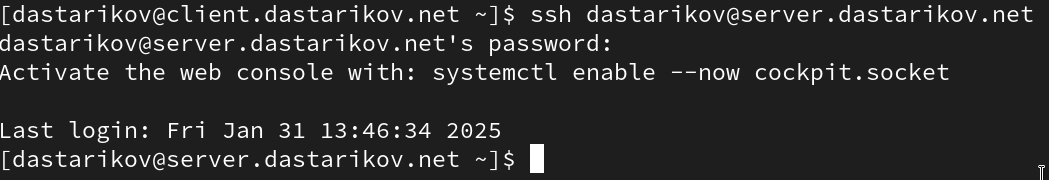
\includegraphics[width=\textwidth]{../images/image03.png}
  \captionof{figure}{Успешное подключение к серверу пользователем dastarikov.}
  \label{03}
\end{center}

\item На сервере открыли файл \texttt{/etc/ssh/sshd\_config} конфигурации \texttt{sshd} на редактирование и добавили строку
  \begin{minted}{bash}
    AllowUsers vagrant
  \end{minted}
\item После сохранения изменений в файле конфигурации перезапустили \texttt{sshd}:
  \begin{minted}{bash}
    systemctl restart sshd
  \end{minted}
\item Повторили попытку получения доступа с клиента к серверу посредством SSH-соединения через пользователя \texttt{dastarikov} (Рис. \ref{04}):
  \begin{minted}{bash}
    ssh dastarikov@server.dastarikov.net
  \end{minted}
\begin{center}
  \centering
  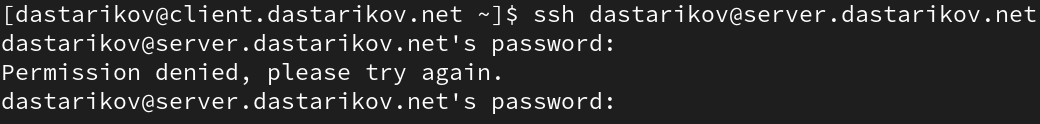
\includegraphics[width=\textwidth]{../images/image04.png}
  \captionof{figure}{Отказ в доступе на сервер пользователю dastarikov.}
  \label{04}
\end{center}

\item В файле \texttt{/etc/ssh/sshd\_config} конфигурации \texttt{sshd} внесли следующее изменение:
  \begin{minted}{bash}
    AllowUsers vagrant dastarikov
  \end{minted}
\item После сохранения изменений в файле конфигурации перезапустили \texttt{sshd} и вновь попытались получить доступ с клиента к серверу посредством SSH-соединения через пользователя \texttt{dastarikov} (Рис. \ref{05}).
\begin{center}
  \centering
  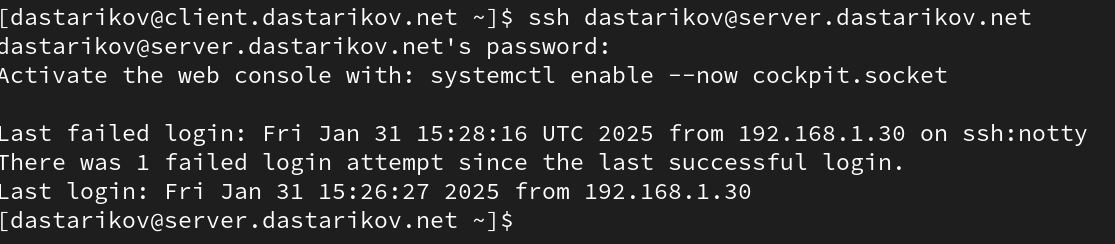
\includegraphics[width=\textwidth]{../images/image05.png}
  \captionof{figure}{Восстановление доступа на сервер пользователю dastarikov.}
  \label{05}
\end{center}

\end{enumerate}
\subsection{Настройка дополнительных портов для удалённого доступа по SSH}
\begin{enumerate}
\item На сервере в файле конфигурации \texttt{sshd /etc/ssh/sshd\_config} нашли строку Port и ниже этой строки добавили:
  \begin{minted}{bash}
    Port 22
    Port 2022
  \end{minted}
  Эта запись сообщает процессу sshd о необходимости организации соединения через два разных порта, что даёт гарантию возможности открыть сеансы SSH, даже если была сделана ошибка в конфигурации.
\item После сохранения изменений в файле конфигурации перезапустили \texttt{sshd}:
  \begin{minted}{bash}
    systemctl restart sshd
  \end{minted}
\item Посмотрели расширенный статус работы \texttt{sshd} (Рис. \ref{06}):
  \begin{minted}{bash}
    systemctl status -l sshd
  \end{minted}
\begin{center}
  \centering
  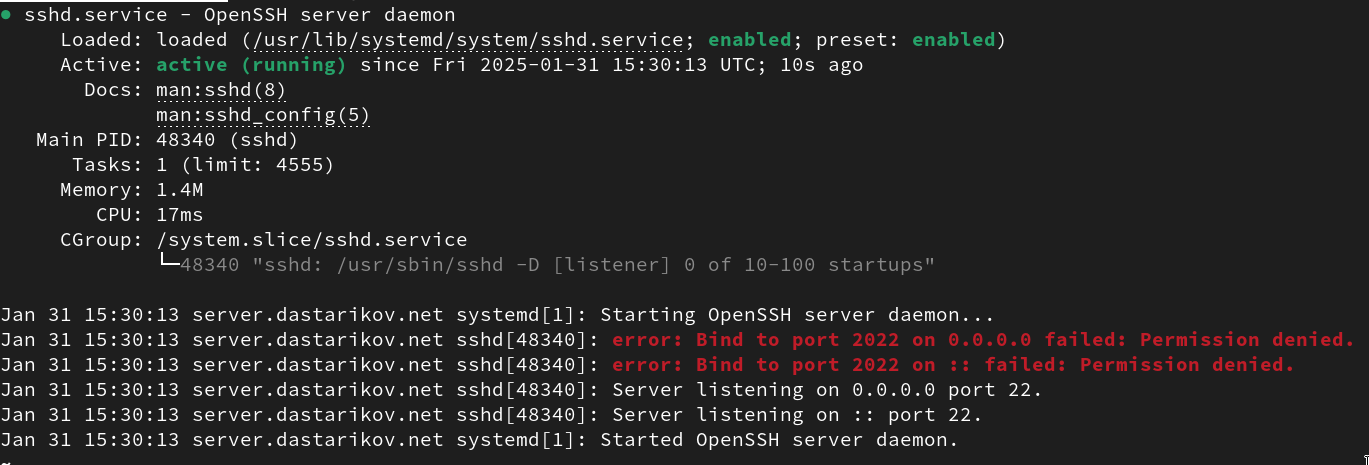
\includegraphics[width=\textwidth]{../images/image06.png}
  \captionof{figure}{Проверка расширенного статуса работы sshd.}
  \label{06}
\end{center}
Видно, что получен отказ в работе sshd через порт 2022. 
\item Исправили на сервере метки SELinux к порту 2022 (Рис. \ref{07}):
  \begin{minted}{bash}
    semanage port -a -t ssh_port_t -p tcp 2022
  \end{minted}
\item В настройках межсетевого экрана открыли порт 2022 протокола TCP (Рис. \ref{07}):
  \begin{minted}{bash}
    firewall-cmd --add-port=2022/tcp
    firewall-cmd --add-port=2022/tcp --permanent
  \end{minted}
\begin{center}
  \centering
  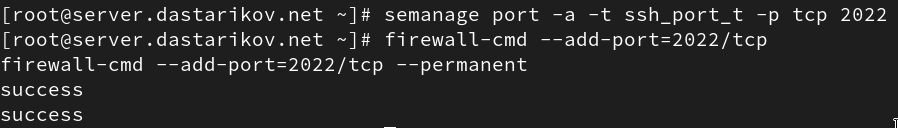
\includegraphics[width=\textwidth]{../images/image07.png}
  \captionof{figure}{Настройка межсетевого экрана.}
  \label{07}
\end{center}

\item Вновь перезапустили \texttt{sshd} и посмотрели расширенный статус его работы. Статус показал, что процесс \texttt{sshd} теперь прослушивает два порта (Рис. \ref{08}).
\begin{center}
  \centering
  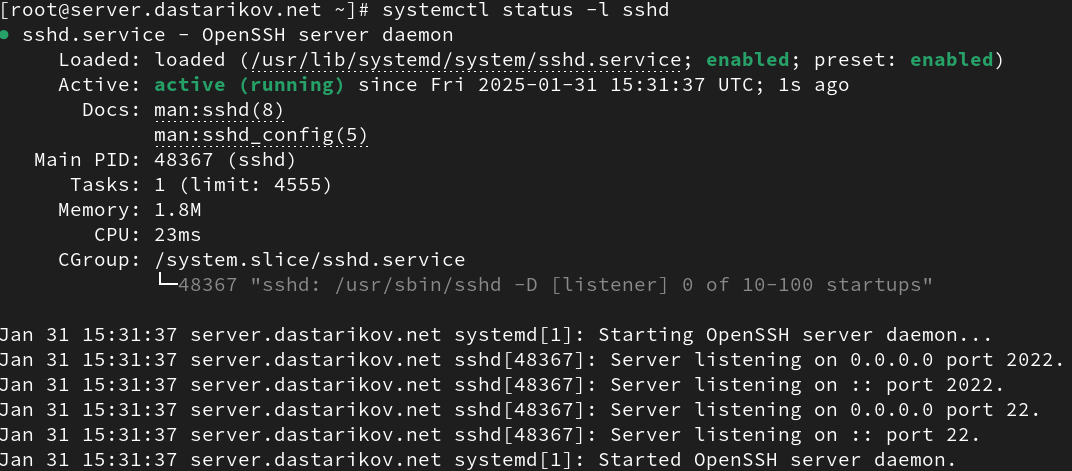
\includegraphics[width=\textwidth]{../images/image08.png}
  \captionof{figure}{Просмотр расширенного статуса sshd после настройки работы с портом 2022.}
  \label{08}
\end{center}

\item С клиента попытались получить доступ к серверу посредством SSH-соединения через пользователя \texttt{dastarikov} (Рис. \ref{09}):
  \begin{minted}{bash}
    ssh dastarikov@server.dastarikov.net
  \end{minted}
  После открытия оболочки пользователя ввели \texttt{sudo -i} для получения доступа \texttt{root}. Отлогинлись от \texttt{root} и пользователя \texttt{dastarikov} на сервере, введя дважды \texttt{logout}  (Рис. \ref{09}).
\begin{center}
  \centering
  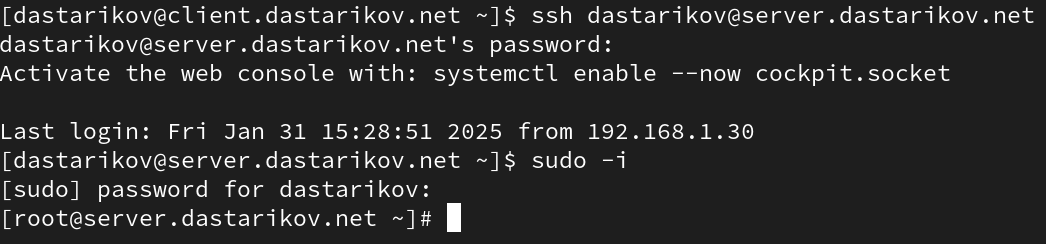
\includegraphics[width=\textwidth]{../images/image09.png}
  \captionof{figure}{Успешное подключение к серверу.}
  \label{09}
\end{center}

\item Повторили попытку получения доступа с клиента к серверу посредством SSH-соединения через пользователя \texttt{dastarikov}, указав порт 2022 (Рис. \ref{10}):
  \begin{minted}{bash}
    ssh -p2022 dastarikov@server.dastarikov.net
  \end{minted}
  После открытия оболочки пользователя ввели \texttt{sudo -i} для получения доступа \texttt{root}. Отлогинлись от \texttt{root} и пользователя \texttt{dastarikov} на сервере, введя дважды \texttt{logout} (Рис. \ref{10}).
\begin{center}
  \centering
  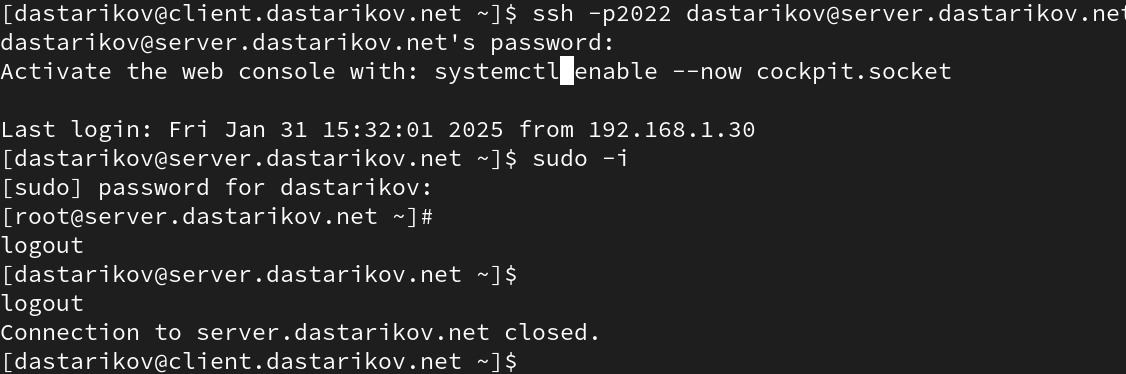
\includegraphics[width=\textwidth]{../images/image10.png}
  \captionof{figure}{Успешное подключение к серверу по порту 2022.}
  \label{10}
\end{center}
\end{enumerate}

\subsection{Настройка удалённого доступа по SSH по ключу}
\begin{enumerate}
\item На сервере в конфигурационном файле \texttt{/etc/ssh/sshd\_config} задали параметр, разрешающий аутентификацию по ключу:
  \begin{minted}{bash}
    PubkeyAuthentication yes
  \end{minted}
\item После сохранения изменений в файле конфигурации перезапустили \texttt{sshd}.
\item На клиенте сформировали SSH-ключ, введя в терминале под пользователем \texttt{dastarikov}:
  \begin{minted}{bash}
    ssh-keygen
  \end{minted}

\item Закрытый ключ был записан в файл \texttt{~/.ssh/id\_rsa}, а открытый ключ записывается в файл \texttt{~/.ssh/id\_rsa.pub}.
\item Скопировали открытый ключ на сервер, введя на клиенте (Рис. \ref{11}):
  \begin{minted}{bash}
    ssh-copy-id dastarikov@server.dastarikov.net
  \end{minted}
  При запросе ввели пароль пользователя на удалённом сервере.
\begin{center}
  \centering
  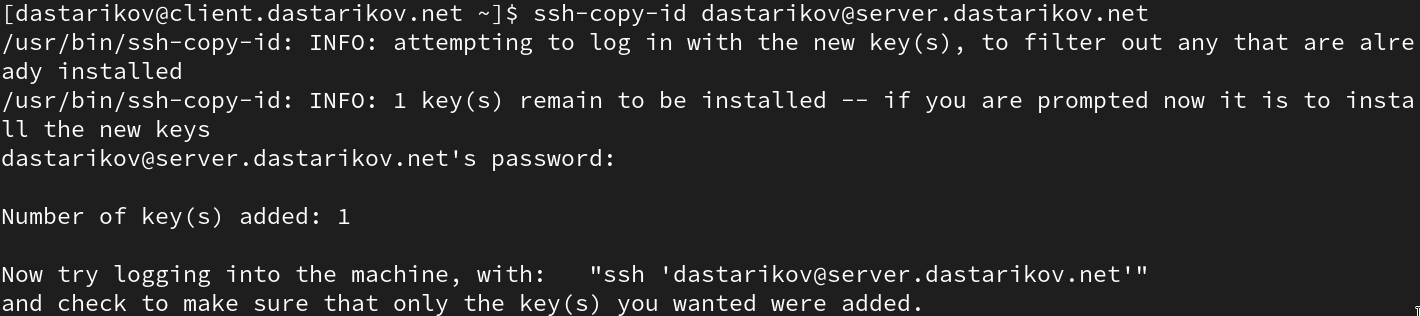
\includegraphics[width=\textwidth]{../images/image11.png}
  \captionof{figure}{Копирование открытого ключа на сервер.}
  \label{11}
\end{center}

\item Попробовали получить доступ с клиента к серверу посредством SSH-соединения (Рис. \ref{12}):
  \begin{minted}{bash}
    ssh dastarikov@server.dastarikov.net
  \end{minted}
  Теперь аутентификация пройдена без ввода пароля для учетной записи удаленного пользователя.
\begin{center}
  \centering
  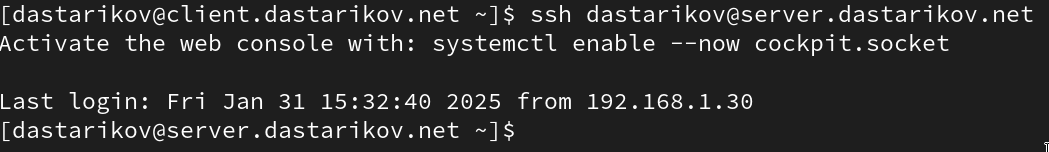
\includegraphics[width=\textwidth]{../images/image12.png}
  \captionof{figure}{Успешное подключение к серверу с использованием SSH-ключа.}
  \label{12}
\end{center}

\end{enumerate}
\subsection{Организация туннелей SSH, перенаправление TCP-портов}
\begin{enumerate}
\item На клиенте посмотрели, запущены ли какие-то службы с протоколом TCP (Рис. \ref{13}):
  \begin{minted}{bash}
    lsof | grep TCP
  \end{minted}
\item Перенаправили порт 80 на \texttt{server.dastarikov.net} на порт 8080 на локальной машине (Рис. \ref{13}):
  \begin{minted}{bash}
    ssh -fNL 8080:localhost:80 dastarikov@server.dastarikov.net
  \end{minted}
\item Вновь на клиенте посмотрели, запущены ли какие-то службы с протоколом TCP (Рис. \ref{13}):
  \begin{minted}{bash}
    lsof | grep TCP
  \end{minted}
\begin{center}
  \centering
  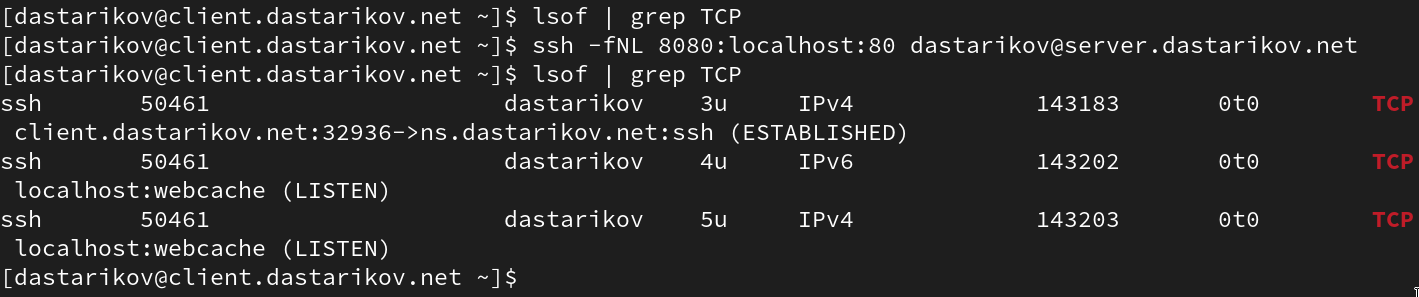
\includegraphics[width=\textwidth]{../images/image13.png}
  \captionof{figure}{Перенаправление TCP-портов.}
  \label{13}
\end{center}

\item На клиенте запустили браузер и в адресной строке введите \texttt{localhost:8080}. Убедились, что отобразится страница с 
приветствием «Welcome to the server.dastarikov.net server».
\end{enumerate}

\subsection{Запуск консольных приложений через SSH}
\begin{enumerate}
\item На клиенте открыли терминал под пользователем \texttt{dastarikov}.
\item Посмотрели с клиента имя узла сервера (Рис. \ref{14}):
  \begin{minted}{bash}
    ssh dastarikov@server.dastarikov.net hostname
  \end{minted}

\item Посмотрели с клиента список файлов на сервере (Рис. \ref{14}):
  \begin{minted}{bash}
    ssh dastarikov@server.dastarikov.net ls -Al
  \end{minted}
\begin{center}
  \centering
  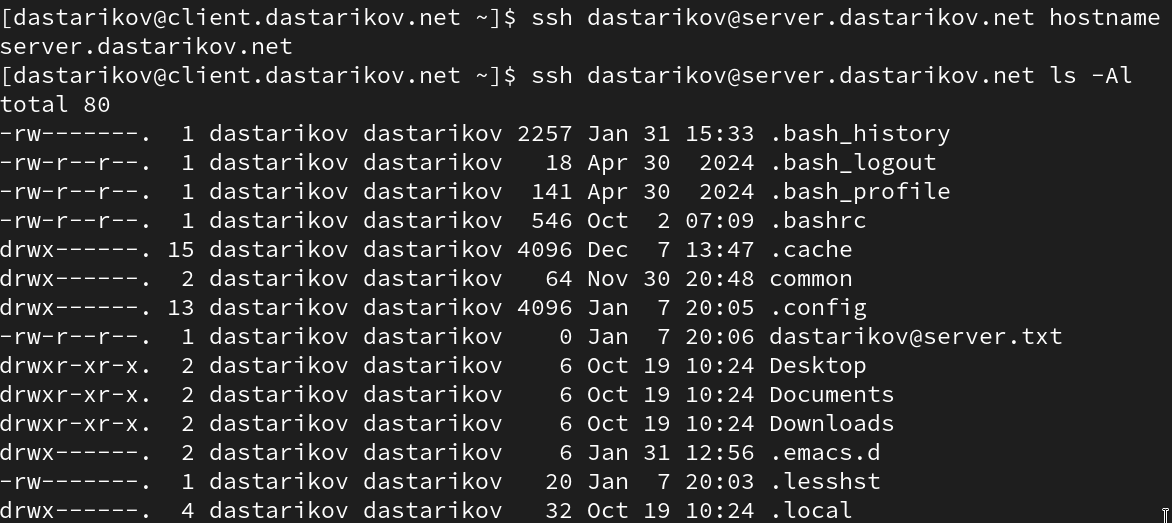
\includegraphics[width=\textwidth]{../images/image14.png}
  \captionof{figure}{Просмотр имени узла сервера и списка файлов через ssh.}
  \label{14}
\end{center}

\item Посмотрели с клиента почту на сервере (Рис. \ref{15}):
  \begin{minted}{bash}
    ssh dastarikov@server.dastarikov.net MAIL=~/Maildir/ mail
  \end{minted}
\begin{center}
  \centering
  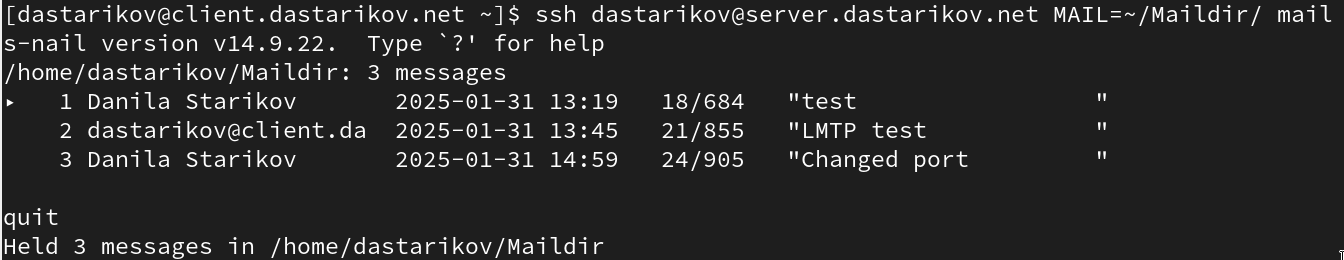
\includegraphics[width=\textwidth]{../images/image15.png}
  \captionof{figure}{Просмотр почты на сервере через ssh.}
  \label{15}
\end{center}

\end{enumerate}
\subsection{Запуск графических приложений через SSH (X11Forwarding)}
\begin{enumerate}
\item На сервере в конфигурационном файле \texttt{/etc/ssh/sshd\_config} разрешили отображать на локальном клиентском компьютере графические интерфейсы X11:
  \begin{minted}{bash}
    X11Forwarding yes
  \end{minted}
\item После сохранения изменения в конфигурационном файле перезапустили \texttt{sshd}.

\item Попробовали с клиента удалённо подключиться к серверу и запустить графическое приложение \texttt{firefox} (Рис. \ref{16}):
  \begin{minted}{bash}
    ssh -YC dastarikov@server.dastarikov.net firefox
  \end{minted}
\begin{center}
  \centering
  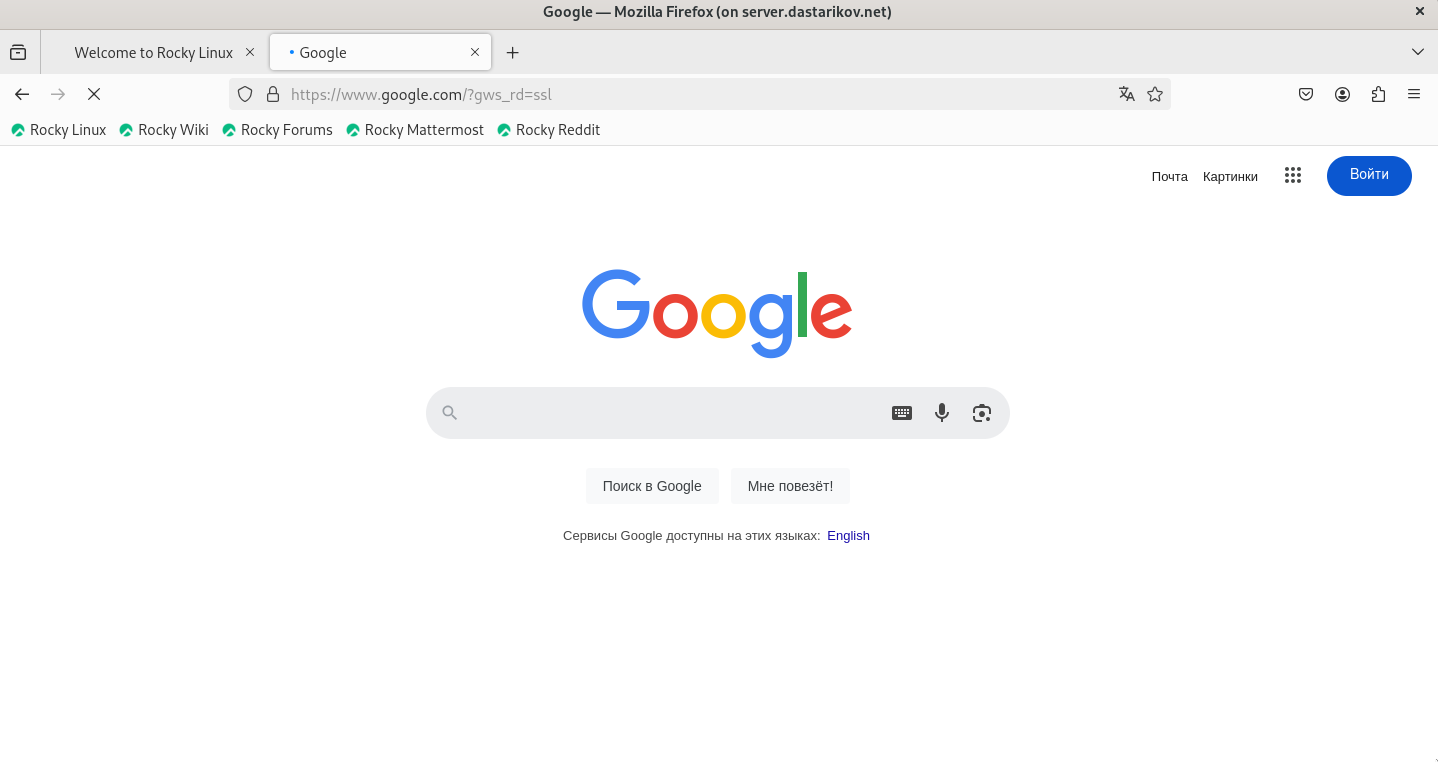
\includegraphics[width=\textwidth]{../images/image16.png}
  \captionof{figure}{Просмотр графического приложения (firefox) через ssh.}
  \label{16}
\end{center}

\end{enumerate}

\subsection{Внесение изменений в настройки внутреннего окружения виртуальной машины}
\begin{enumerate}
\item На виртуальной машине \texttt{server} перешли в каталог для внесения изменений в настройки внутреннего окружения \texttt{/vagrant/provision/server/}, создали в нём каталог \texttt{ssh}, в который поместите в соответствующие подкаталоги конфигурационный файл \texttt{sshd\_config}:
  \begin{minted}{bash}
    cd /vagrant/provision/server
    mkdir -p /vagrant/provision/server/ssh/etc/ssh
    cp -R /etc/ssh/sshd_config /vagrant/provision/server/ssh/etc/ssh/
  \end{minted}
\item В каталоге \texttt{/vagrant/provision/server} создали исполняемый файл \texttt{ssh.sh}:
  \begin{minted}{bash}
    cd /vagrant/provision/server
    touch ssh.sh
    chmod +x ssh.sh
  \end{minted}
  Открыв его на редактирование, прописали в нём следующий скрипт:
  \begin{minted}{bash}
    #!/bin/bash
    echo "Provisioning script $0"
    echo "Copy configuration files"
    cp -R /vagrant/provision/server/ssh/etc/* /etc
    restorecon -vR /etc
    echo "Configure firewall"
    firewall-cmd --add-port=2022/tcp
    firewall-cmd --add-port=2022/tcp --permanent
    echo "Tuning SELinux"
    semanage port -a -t ssh_port_t -p tcp 2022
    echo "Restart sshd service"
    systemctl restart sshd
  \end{minted}
\item Для отработки созданного скрипта во время загрузки виртуальной машины \texttt{server} в конфигурационном файле Vagrantfile добавили в разделе конфигурации для сервера:
  \begin{minted}{bash}
    server.vm.provision "server ssh",
    type: "shell",
    preserve_order: true,
    path: "provision/server/ssh.sh"
  \end{minted}
\end{enumerate}


\section{Выводы}
В результате выполнения лабораторной работы приобрели практические навыки по настройке удалённого доступа к серверу с помощью SSH.
\end{document}
